\section{Diagramas}
\subsection{Diagramas de Clases (UML)}
Para entender correctamente la relación entre las clases, tanto de las ya dadas en el fichero original como de las creadas posteriormente, se ha realizado un diagrama de clases en formato \emph{UML} para ello se ha empleado el programa StarUML\textsuperscript{\textregistered}.

\begin{figure}[h]
    \centering
    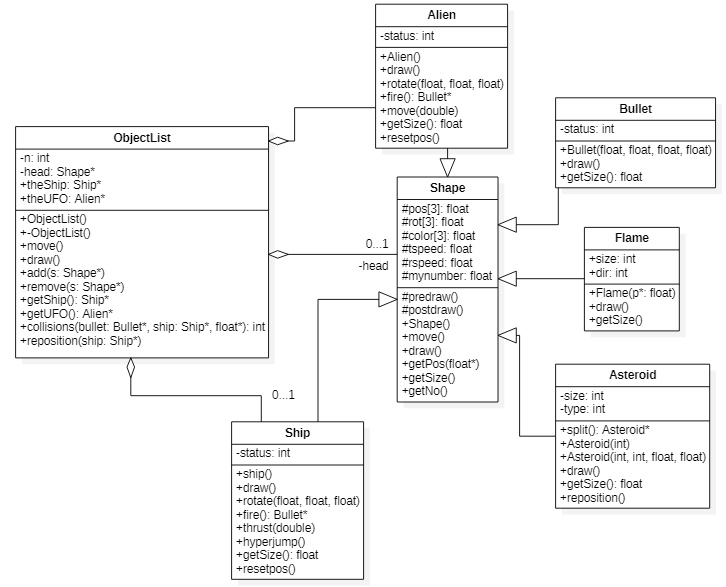
\includegraphics[width=\textwidth]{fotos/UML.PNG}
    \caption{Diagrama de clases del juego mediante \emph{StarUML}}
    \label{uml}
\end{figure}

Como puede verse en la Ilustración \ref{uml}, la clase \emph{ObjectList} agrega punteros a las clases \emph{Alien}, \emph{Ship} y \emph{Angel}, además de contener un puntero tipo \emph{Shape} llamado \textit{head} que apunta a la cabeza de la lista (pero que en la implementación realizado no se utiliza). Al igual que la clase \emph{Ship}, las clases \emph{Alien}, \emph{Angel}, \emph{Bullet}, \emph{Flame} y \emph{Asteroid} son hijas de la clase \emph{Shape}. La clase \emph{Alien} tiene mucho en común con la clase \emph{Ship}, pues realizan prácticamente lo mismo, con la diferencia de que el OVNI (instancia de la clase \emph{Alien}) se mueve automáticamente y de forma errática sin ser necesaria la interacción con el usuario. Por comodidad se han añadido dos punteros, uno al OVNI y otro a la astronave (\emph{theShip}), que simplificarán mucho el código tanto en la lógica del juego como en la implementación de la clase \emph{ObjectList}.
A parte de las clases aquí representadas, existe otro archivo de cabecera llamado \emph{commonstuff}, que almacena funciones cortas, parámetros y llamadas a librerías usadas en todos los archivos fuente del programa.
\subsection{Diagramas de comunicación}

El siguiente diagrama ilustra desde dónde se crean los objetos que se van a usar en el resto del programa:

\begin{figure}[h]
    \centering
    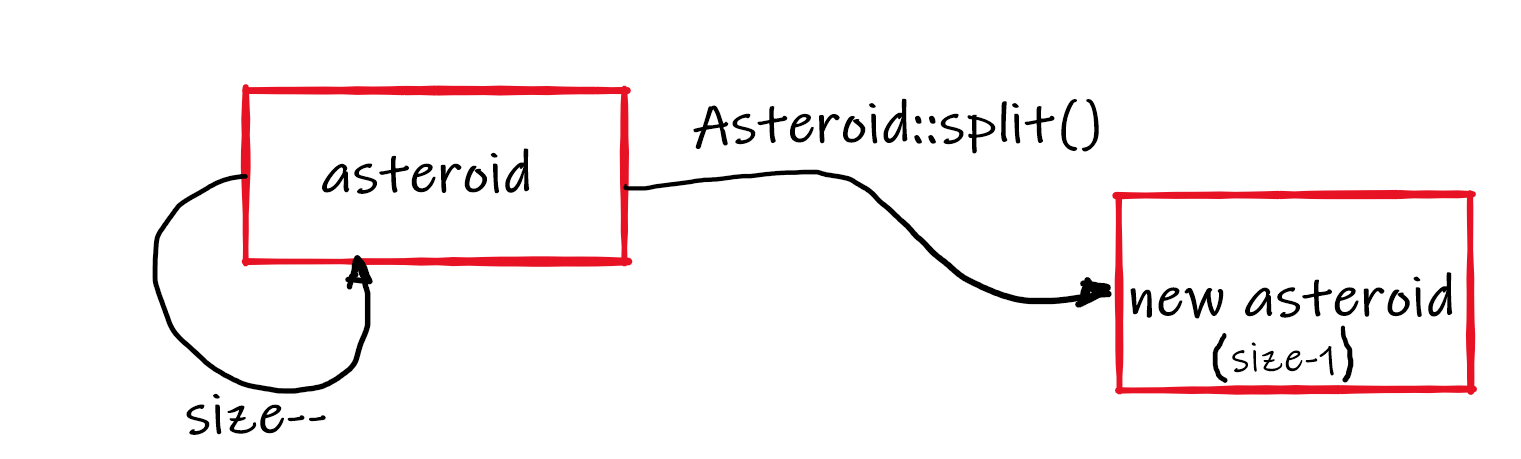
\includegraphics[width=\textwidth]{fotos/asteroid.png}
    \caption{Diagrama de comunicación }
    \label{asteroid}
\end{figure}

El diagrama de la Ilustración \ref{asteroid} representa el mecanismo de creación de los objetos más importantes que se lleva a cabo en el constructor del objeto \emph{ObjectList} y la creación de la bala a través del método \textsc{fire()} del objeto \emph{theShip}. Se crean también todos los asteroides, donde su número concreto viene definido por el parámetro \textsc{NUMASTEROIDS} definido en \emph{commonstuff.hpp}. Los asteroides son inmediatamente cargados en la interfaz gráfica mediante la función $push_front()$ de la plantilla $<list>$, a diferencia del OVNI (\emph{theUFO}), que será cargado desde la lógica del juego cuando se cumplan las condiciones especificadas en el algoritmo.
A continuación, en otro pequeño diagrama de objetos, se verá el comportamiento de uno de los objetos \emph{Asteroid} cuando es impactado por una bala o por la astronave.
